\chapter{Towards OWL-aware similarity} \label{chap:enhancements}

The biomedical informatics community is actively committed to the adoption of formal-logic knowledge representation languages, such as the Web Ontology Language (OWL), and the use of reference ontologies to annotate biomedical resources (\cf \appref{app:ontologies}). This adoption has resulted in the increase of
\begin{paralist}
    \item the amount of knowledge represented in ontologies, and
    \item the quality of these representations in respect to the reality.
\end{paralist}

As has been argued by \citet{Couto2013}, there are some benefits to considering exploiting formal axioms in the calculation of semantic similarity. In this chapter, I report the enhancements that I achieved in the pursuit of semantic similarity measures that can maximise the use of these axioms. I first report on a measure that can use disjointness axioms and then on another that can use existential quantifications.


\section{Disjointness axioms in semantic similarity} \label{sec:enhancements/disjointness}

\begin{note-paper}
    This section is adapted from a paper produced in collaboration with Janna Hastings from the European Bioinformatics Institute, published in Oxford Bioinformatics~\citep{Ferreira2013}.
\end{note-paper}


\subsection{The idea}

Disjointness axioms are one example of formal constructions in OWL ontologies that are gaining momentum in the biomedical informatics community. For example, the Chemical Entities of Biological Interest (\ontology{CHEBI}) ontology now includes this type of axioms~\citep{Hastings2013}. To explore this new type of information, I devised an algorithm that can be \emph{plugged} into some semantic similarity measures to take into account disjointness information.

A disjointness axiom declared for a pair of concepts express the constraint that an instance of one of them cannot also be an instance of the other. This constraint logically implies that the two concepts cannot have common subclasses. Should such shared subclasses be detected by a reasoner, the reasoner will flag the ontology as \emph{inconsistent}~\citep{Sattler2013}, which can be used by ontology developers to prevent errors in ontology development. For example, in \ontology{CHEBI}, this technique has been used to detect that a specific ion (a type of charged molecule) was misclassified as a group (a strict part of a molecule)~\citep{Hastings2012}.

\begin{figure}
    \centering
    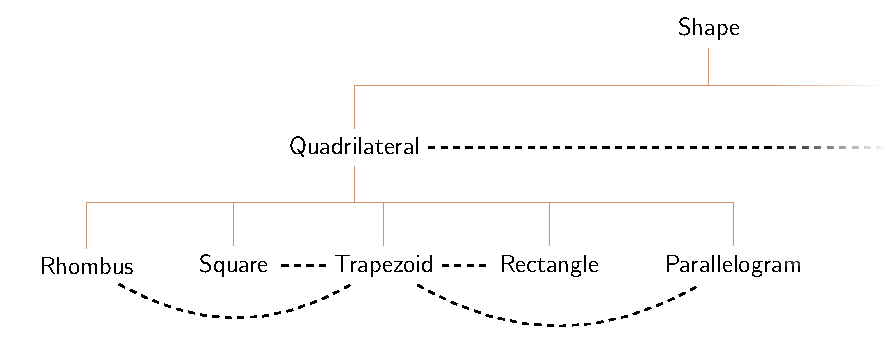
\includegraphics[width=\textwidth]{images/shape-ontology.pdf}
    \caption[A snippet of a hypothetical Shape Ontology]{In this snippet, I use the term \term{Parallelogram} as ``a quadrilateral with two pairs of parallel sides'' and \term{Trapezoid} to mean ``a quadrilateral with two parallel sides and two obtuse angles''. Solid lines represent class-subclass relationships, dashed lines represent disjointness axioms. Note that a proper shape ontology would classify \term{Square} as a subclass of \term{Rectangle}, \term{Rhombus} and \term{Parallelogram}, and \term{Rhombus} as equivalent to \term{Parallelogram}. For the sake of the argument being exposed, however, assume that such information is yet unknown by the ontology creators.}
    \label{fig:shape}
\end{figure}

\figref{fig:shape} illustrates this situation: this ontology snippet asserts that no instance of \term{Rectangle} can simultaneously be an instance of \term{Trapezoid}. However, given the open-world assumption that underlies OWL ontologies (see \secref{sec:concepts/ontologies}), there can be instances of \term{Rectangle} that are also instances of \term{Parallelogram} (in fact, it is a consequence of the relevant geometric definitions that squares are both rectangles and parallelograms). For this reason, the similarity between \term{Rectangle} and \term{Parallelogram} should intuitively be higher than the similarity between \term{Rectangle} and \term{Trapezoid}. Using $\sigma$ to represent the function that returns the similarity between two concepts, this hypothesis can be mathematically stated with \eqref{eq:motivation}:
\begin{equation}
    \sigma(\term{Rectangle}, \term{Parallelogram}) >
    \sigma(\term{Rectangle}, \term{Trapezoid}).
    \label{eq:motivation}
\end{equation}


\subsection{The proposed measure} \label{sub:disjointness/measure}

As has been discussed in \secref{sec:sota/node}, there has been an effort to design measures that compute the shared information content between two concepts: while shared information content between concepts $x$ and~$y$ has been assumed to be well estimated by the maximal information content of the concepts that subsume both $x$ and~$y$, \citet{Couto2011} suggest DiShIn, a shared information content measure that builds upon existing measures (such as the ones in \eqref{eq:resnik-ssm,eq:lin}) and which behaves as a \emph{plug-in} to such measures. In its particular case, DiShIn explores \emph{multiple parentage} in order to ensure that all shared information across multiple ancestors is taken into account.

Likewise, instead of developing a new semantic similarity measure to deal with disjointness axioms, I proposed a \emph{plug-in} to be used on top of existing measures of shared information content. My \emph{plug-in} refines the estimation of shared information between two concepts by incorporating the disjointness axioms asserted in the ontology. In here, I denote the disjointness-aware measure of shared information content between concepts $x$ and~$y$ as $\ICsdis(x,y)$, which is calculated based on an existing measure of shared information content,~$\ICs(x,y)$.

Given the example presented in \figref{fig:shape} and the inequality of \eqref{eq:motivation}, it would be desirable for the measure of shared information content to decrease for concepts that are known to be disjoint, formalising the intuition that disjoint concepts are less similar because they cannot share subclasses. Furthermore, to respect the open-world assumption, the measure should stay unchanged when two concepts are \emph{not known} to be disjoint.

With these constraints in mind, I proposed the following measure of shared information content:
\begin{equation}
    \ICsdis(x,y) = \ICs(x,y) - k(x,y)
    \label{eq:new-disj}
\end{equation}
where $\ICs(x,y)$~is any measure of shared information content between $x$ and~$y$, $k(x, y) > 0$ if $x$ and~$y$ are disjoint and $k(x, y) = 0$ otherwise.

\begin{figure}
    \centering
    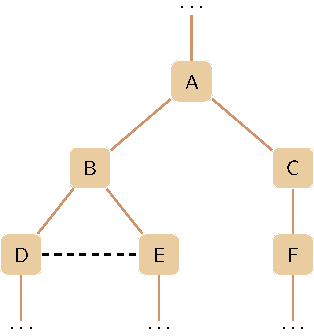
\includegraphics[width=0.35\textwidth]{images/toy-disjoints.pdf}
    \caption[Example ontology with disjointness axioms]{This illustrates a toy ontology that shows some concepts in a class-subclass hierarchy (represented with solid lines) as well as a disjointness axiom asserted between two concepts (dashed lines).}
    \label{fig:toy}
\end{figure}

Two points were crucial in the development of this measure. First, note that, as is, this equation presents a \emph{discontinuity}. In the hypothetical ontology of \figref{fig:toy}, this measure implies
\begin{equation}
    \ICsdis(\term D, \term E) < \IC(\term B),
\end{equation}
which, depending on the value $k(\term D, \term E)$, could lead to
\begin{equation}
    \ICsdis(\term D, \term E) < \IC(\term A) = \ICsdis(\term D, \term F).
\end{equation}
However, this should not be possible, since \term D and \term E share more information than \term D and~\term F. Therefore, $k$ must be bounded according to the $\IC$ of the most informative ancestor of the $\MICA$, which, in this case, results in
\begin{equation}
    k(\term D, \term E) \leq \IC(\term B) - \IC(\term A).
\end{equation}

\begin{figure}
    \centering
    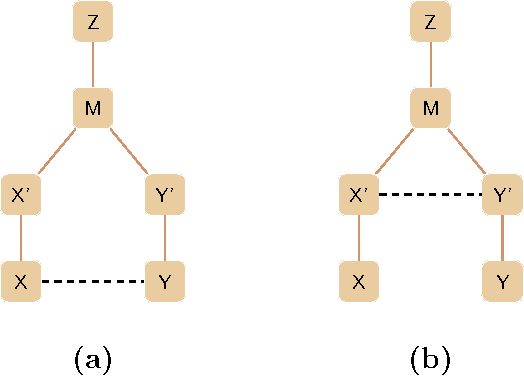
\includegraphics[width=0.594\textwidth]{images/strength.pdf}
    \caption[The potential for implicit common superclasses between two concepts]{In both cases, $\MICA(\term X, \term Y) = \term M$, and the most informative ancestor of \term M is \term Z. The difference is in the location of the disjointness axiom. In situation A, there is a higher likelihood of implicit common ancestors (ICA) between \term X and~\term Y, because the axiom of disjointness is further down from their common ancestry.}
    \label{fig:strength}
\end{figure}

The second major decision in the development of this measure is related to an operational notion. In fact, I have not yet defined how to compute~$k(x,y)$. I propose an algorithm based on the notion of potential for \emph{implicit common superclasses} (ICS), which measures the likelihood that two concepts share non-asserted superclasses. Consider the ontology snippets in \figref{fig:strength}. In situation~A, given the open-world assumption, there is a small chance that \term Y turns out to be a subclass of~$\term{X'}$, while in situation~B that cannot happen, since \term Y is inferred to be disjoint with~$\term X'$ (the disjointness axiom is higher up in the hierarchy). This suggests that there is a higher potential for ICS between the concepts \term X and~\term Y in situation~A.

I model the \emph{unlikelihood} of ICS as~$f(x, y)$, a function that returns higher values for situations with lower potential for ICS:
\begin{equation}
    f(x, y) =
    \max\left\{
        \frac{1}{p(a,b)} \,\Big|\, a\in\anc(x) \wedge b\in\anc(y) \wedge J(a,b)
    \right\}\cup\{0\}
\label{eq:strength}
\end{equation}
where $\anc(c)$~is the set of superclasses of~$c$ (including~$c$), $J(a, b)$~is true when $a$ and~$b$ are disjoint (either by assertion or inference) and false otherwise, and $p(a, b)$~is the edge length of the shortest path from $a$ to~$b$, taking into account only class-subclass relationships, not the disjointness arcs (only the solid edges in the figures, not the dashed ones).

Using the example ontologies in \figref{fig:strength}, we can illustrate this definition by calculating~$f(\term X, \term Y)$. In A, $J(a,b)$~is true only for $(a,b)=(\term X, \term Y)$; the shortest path from \term X to~\term Y is $\term X \rightarrow \term{X'} \rightarrow \term M \rightarrow \term{Y'} \rightarrow \term Y$, which has length~$4$. Therefore,
\begin{equation}
    f(\term X, \term Y)=\max\left\{\frac14,0\right\}=\frac14.
\end{equation}

In B, $J(a,b)$~is true for $(a,b)\in\{(\term X, \term Y), (\term X, \term{Y'}), (\term{X'}, \term Y), (\term{X'}, \term{Y'})\}$. These correspond to paths of length $4$, $3$, $3$ and~$2$, respectively, leading to
\begin{equation}
    f(\term X, \term Y) = \max\left\{\frac14, \frac13, \frac12, 0\right\}=\frac12.
\end{equation}

Additionally, in situation A, $f(\term{X'}, \term{Y'}) = 0$, since the two concepts are not disjoint and as such $J(a,b)$~is always false.

The general procedure to calculate $\ICsdis(x,y)$ is, therefore:
\begin{enumerate}
    \item Determine $M = \MICA(x,y)$
    \item Determine $Z = \argmax_c \{\IC(c)\,|\,c\in\anc(M)\}$, \ie the most informative ancestor of~$M$;
    \item Calculate $f(x, y)$, as described in \eqref{eq:strength};
    \item Calculate $k(x,y) = f(x,y)\cdot(\IC(M) - \IC(Z))$;
    \item Calculate $\ICsdis(x,y)=\ICs(x,y)-k(x,y)$.
\end{enumerate}

With this procedure, the new shared information content is estimated as a weighted average between $\IC(M)$ and~$\IC(Z)$, where a low potential for ICS leads to a shared information content close to~$\IC(Z)$ and a higher potential for ICS leads to a shared information content close to~$\IC(M)$. This means that the shared information content decreases by a larger amount when there is a smaller potential for implicit common superclasses. Note that if the two concepts are not disjoint, $k(x,y)=0$ and $\ICsdis=\ICs$, which satisfies the open-world assumption mentioned previously.


\subsection{Validation}

According to the hierarchy presented in \chpref{chap:validation}, I classify the validation approach followed in this work as a ``Comparison with an anchor measure''. For this purpose, I calculated structural similarity between \ontology{CHEBI} concepts (details can be found on the paper), and semantic similarity using the algorithm described above, and measured the Pearson's correlation coefficient between the two measures.

The proposed measure was validated in three steps, by measuring the increase in coefficient
\begin{paralist}
    \item in the presence \vs absence of disjointness axioms,
    \item with increasing fractions of the total number of disjointness axioms, and
    \item in several random datasets.
\end{paralist}

For a fully detailed discussion of these three steps, I refer the reader to the published paper. Here I summarise the main results.

\point{Increase in correlation coefficient} I applied the new measure of shared information content to a subset of \ontology{CHEBI}, including some disjointness axioms~\citep{Hastings2012,Hastings2013}. Since it consists of a \emph{plug-in} and relies on a previously defined measure of shared information content, I used, in this assessment, the classical notion of shared information content proposed by~\citet{Resnik1995}:
\begin{equation}
    \ICs(x,y) = \IC(\MICA(x,y))
\end{equation}
where information content was calculated using \eqref{eq:seco}.

Given the sparsity of disjointness axioms relative to the size of \ontology{CHEBI}, random pairs of concepts would rarely touch any disjointness information and it would be difficult to detect the difference resulting from these axioms. As such, the concepts in the dataset were chosen so that a significant part of them had disjointness information. Additionally, given the need to calculate structural similarity, the concepts in the dataset were also selected in order to ensure that structural similarity was possible. While these two constraints slightly bias the generated dataset, I believe that the bias did not result in a dataset too different from reality: in fact, although the amount of disjointness axioms already added to \ontology{CHEBI} is not high, true disjointness exists for most pairs of concepts.

Structural similarity was calculated using PubChem's fingerprint method~\citep{Bolton2008}. Structural similarity between \ontology{CHEBI} concepts that do not represent actual molecules but rather chemical groups (\eg there is not a single chemical structure for \term{Hexose} but rather a collection of them) was achieved by comparing the collection of structures.

For the dataset created above, I compared all compounds with all
the other compounds using three measures: structural similarity, classical $\ICs$ and~$\ICsdis$. I used Wolfe's t-Test~\citep{Wolfe1976,Rosner2010} to determine the statistical significance of the increase in the correlation coefficient between the pair~$(\textrm{structural}, \ICs)$ and the pair~$(\textrm{structural}, \ICsdis)$.

The Pearson's correlation coefficient between the structural measure and~$\ICs$ is~$0.69883$, and after taking the disjointness axioms into account, the correlation between structural similarity and~$\ICsdis$ becomes~$0.71571$. This represents an increase of~$0.01688$. Despite the small absolute increase, this value is statistically significant, with a~\emph{p}-value of~$4.5 \times 10^{-8}$. The small increase of the correlation can be attributed to at least three
factors:
\begin{itemize}
    \item As the annotation of disjointness is still incomplete in \ontology{CHEBI}, we have access to only a small subset of all the \emph{real} disjointness axioms that can be expressed in \ontology{CHEBI}, which means that the shared information content changes only for a fraction of all the concept pairs ($39\%$ of the pairs in the dataset). I expect that, as the number of disjointness axioms added to \ontology{CHEBI} increases, both this fraction and the difference between correlation coefficients will increase.
    \item While highly correlated, structural similarity and semantic similarity measures are inherently different, and as such there is a maximum bound on the actual correlation that can be expected between the two (\cf \secref{sub:hierarchy/comparison}).
    \item Disjointness is only one of the logical axiom types that are used to express concept definitions in an OWL ontology. In fact, \ontology{CHEBI} contains a number of other properties that are also used to capture the meaning of its concepts, \eg the property \prop{has-tautomer}, which connects together closely structurally related chemicals, and \prop{has-role}, which connects a chemical concept to its biological activity.
\end{itemize}


\point{Effect of the number of axioms} The second assessment step measured the effect of the number of disjointness axioms on the correlation coefficient. I partitioned the $199$~disjoitness axioms into $10$~sets: the first contained $20$~random axioms, the second contained these plus another $20$~random axioms, \etc., with the final one containing the $199$~axioms (see \figref{fig:partitions}). For each set, I calculated $\ICsdis$ on the previous dataset and plotted a graph showing the increase in correlation \vs the number of axioms. To remove any bias that resulted from the random method used to partition the axioms, I repeated this process $20$~times.

\begin{figure}
    \centering
    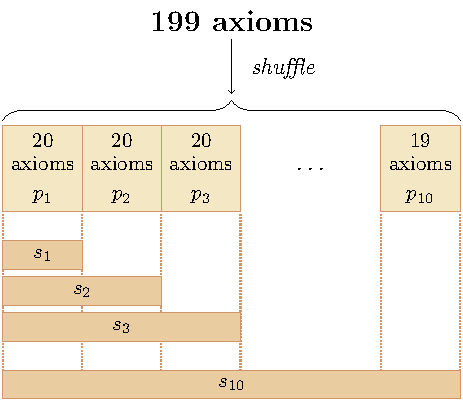
\includegraphics[width=0.6\textwidth]{images/partition.pdf}
    \caption[Partitioning the set of disjointness axioms]{The process used to assess the effect of the number of axioms on the correlation coefficient between structural and semantic similarity. The axioms are randomly partitioned into clusters $p_1$ to~$p_{10}$. Consecutively, each of these clusters is joined with the previous ones to create the sets $s_i = \bigcup_{j=1}^i p_j$, which are then used to compute the increase in correlation coefficient.}
    \label{fig:partitions}
\end{figure}

This validation step has the objective of simulating the development of \ontology{CHEBI} ontology with respect to the number of disjointness axioms. For each of the $20$~repetitions, I studied the difference between the correlation coefficients as the number of disjointness axioms increases, and plotted a graph with this information.

The graphs in \figref{fig:evolution} show the result of some of these repetitions. These graphs illustrate that not all disjointness axioms are important for a given dataset. In fact, only for some of the sets of axioms is the correlation coefficient significantly affected, which suggests that those sets contained the axioms that change the logical meaning behind the concepts in the dataset. The graphs present an obvious trend (see \figref{fig:evolution-trend} for an average of the graphs of all the $20$~repetitions) that indicates an increase of the correlation, which, again, indicates that the disjointness axioms improve the correctness of semantic similarity.

\begin{figure}
    \centering
    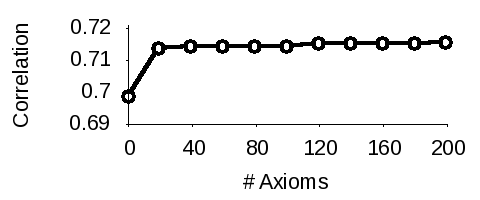
\includegraphics[width=0.4\textwidth]{images/plot18.png}
    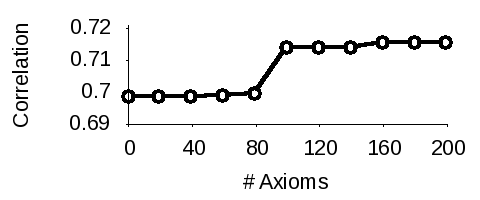
\includegraphics[width=0.4\textwidth]{images/plot17.png}
    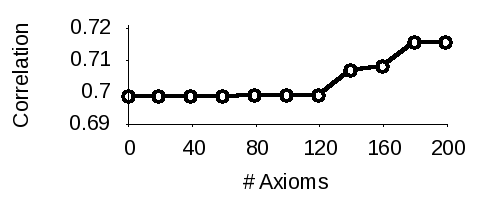
\includegraphics[width=0.4\textwidth]{images/plot3.png}
    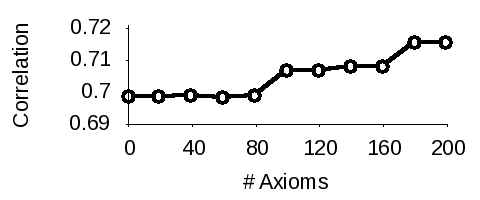
\includegraphics[width=0.4\textwidth]{images/plot1.png}
    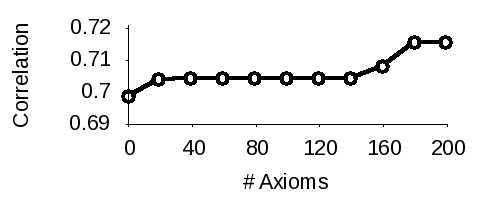
\includegraphics[width=0.4\textwidth]{images/plot10.png}
    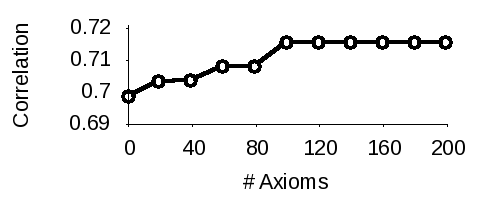
\includegraphics[width=0.4\textwidth]{images/plot8.png}
    \caption[The effect of increasing number of disjointness axioms]{These graphs illustrate the increase in correlation coefficient that results from increasing the number of disjointness axioms. In each graph, the abscissa is the number of axioms used by the semantic similarity measure and the ordinate is the correlation coefficient. The correlation coefficient for $0$~axioms is always equal to the correlation measured with the classical~$\ICs$, which is~$0.69883$; the correlation coefficient for the maximum number of axioms corresponds to the value~$0.71571$, presented in the first validation step. These graphs are representative of the behaviour obtained in all the $20$~repetitions.}
    \label{fig:evolution}
\end{figure}

\begin{figure}[p]
    \centering
    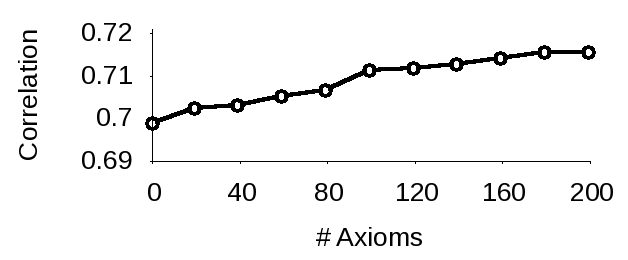
\includegraphics[width=0.6\textwidth]{images/trend.png}
    \caption[The trend corresponding to all the repetitions]{This graph shows the average of all the graphs produced in the $20$~repetitions. Although these values do not have any statistical significance in themselves, they clearly show the trend that the more disjointness axioms are considered, the better is the correlation between structural and semantic similarity.}
    \label{fig:evolution-trend}
\end{figure}


\point{Effect on other datasets:} As the third assessment step, I studied the increase in correlation coefficient on other datasets, since the dataset created for the first step resulted from a random selection process. Following the same selection process, I created $550$~more datasets and compared the correlation coefficient as previously explained.

The graph of \figref{fig:histogram} shows an histogram that represents the difference in the Pearson's correlation coefficient for all these datasets. As is visible in that graph and in \tabref{tab:histogram}, the vast majority of the datasets are associated with an increase in the correlation coefficient. In fact, the effect of considering the disjointness axioms for the semantic similarity only impacts negatively $6.2\%$ of the datasets. We observed a mean correlation increase of~$0.0149$, with a standard deviation for that value of~$0.0130$. Furthermore, in $72.5\%~$of the datasets, the increase in correlation is significant at a confidence value of $0.05$.

\begin{figure}[p]
    \centering
    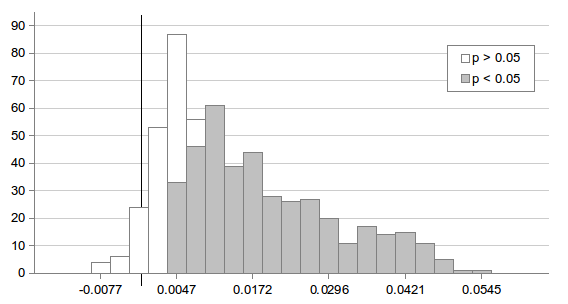
\includegraphics[width=0.7\textwidth]{images/histogram.png}
    \caption[Distribution of the difference in correlation coefficient for random datasets]{The majority of the cases show a positive difference. I used Wolfe's t-Test to calculate the \emph{p}-value associated with the hypothesis that the increase was due to random chance, and marked with a darker shade the amount of datasets for which p-value${}<0.05$. The vertical line shows the zero of the axis, \ie where the two correlation coefficients are the same.}
    \label{fig:histogram}
\end{figure}

\begin{table}[p]
    \centering
    \small
    \caption[Statistics related to the histogram of \figref{fig:histogram}]{The last column shows the frequency relative to all the datasets created.}
    \begin{tabular}{lrr}
    \toprule
        & \bfseries \# datasets & \bfseries \% datasets \\
    \midrule
    Increase in correlation & 516 &  93.8\% \\
    p-value${}<0.05$        & 399 &  72.5\% \\
    \bottomrule
    \end{tabular}
    \label{tab:histogram}
\end{table}


\subsection{Limitations, future work and other conclusions}

This measure has some limitations:
\begin{enumerate}
    \item The formula of~$\ICsdis$ is not robust against ontology development. Sometimes, the addition of a concept to the ontology during development can considerably change the value of shared information content between two concepts (\cf \secref{sub:hierarchy/theoretical}, where I mention this problem in the context of semantic similarity validation). This issue is mitigated by the fact that the such additions are not common in biomedical ontologies (full details in the paper).
    \item The potential for implicit common superclasses is measured using an edge distance, which is a fragile measure in biomedical ontologies~\citep{Pesquita2009} (see \secref{sec:sota/edge}). It may be possible to explore the semantics of the edges themselves in order to overcome this issue.
    \item The measure of information content influences the results obtained with~$\ICsdis$. In this case, IC was calculated with an intrinsic measure of information content; it would be informative to see the effect of changing the IC measure to an extrinsic one.
\end{enumerate}

This validation shows that considering disjointness axioms improves the shared information content measure, with statistical significance. This new approach is able to successfully explore more than just the class-subclass hierarchy of an ontology, relying on a partial subset of the description logic axioms that are included in the ontology to refine the comparison algorithm. To the best of my knowledge, this represents the first attempt to explicitly use description logic expressivity in semantic similarity in the biomedical domain. I demonstrated this hypothesis using a rather naïve approach. More sophisticated approaches include the exploration of the semantics of edges, other types of information content based on external corpus, \etc.

\section{Semantic relatedness measure} \label{sec:enhancements/relatedness}

\begin{note-paper}
    This section is adapted from a papers accepted for oral presentation at the International Conference on Biomedical Ontology~2011 and published in the corresponding proceedings~\citep{Ferreira2011}.
\end{note-paper}

\subsection{The idea}

According to the definition provided in \secref{sec:concepts/semantic-similarity}, semantic similarity uses exclusively the hypernymy relationship of an ontology: the class-subclass hierarchy. In this sense, \term{Heart} and \term{Blood} are not similar at all. However, in some contexts, hypernymy is not enough to detect that two concepts are related to one another. Anatomy, specifically when used to detect similarity between diseases, is one of these contexts. For example, a heart disease can have implications in blood pressure, and thus a disease annotated with the concept \term{Heart} is somewhat related to one annotated with the concept \term{Blood}.

\begin{figure}[!b]
    \centering
    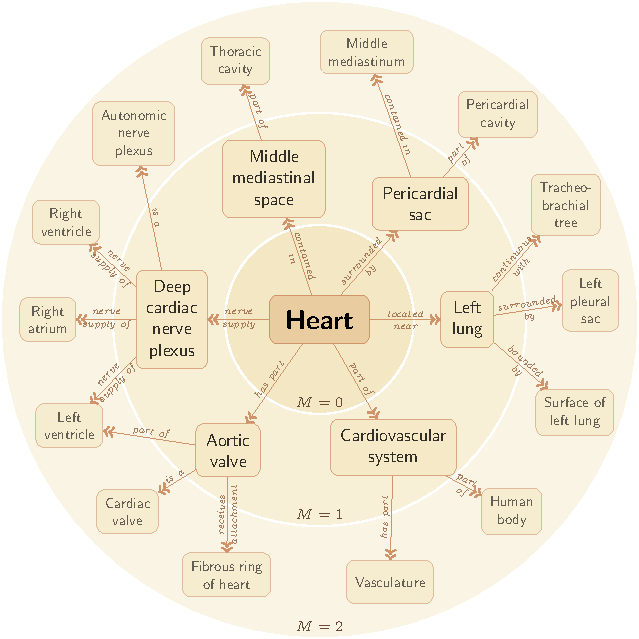
\includegraphics{images/heart-neighbourhood.pdf}
    \caption[The semantic neighbourhood of the concept \term{Heart}]{This picture illustrates the semantic neighbourhood of \term{Heart}, with a radius~$M=2$. As depicted, \term{Aortic valve} is part of the first layer since it directly links to \term{Heart}, while \term{Cardiac valve} is part of the second layer. Notice that some neighbours can be connected to the centre by more than one distinct path (\eg \term{Left ventricle}). The \emph{radius} can be increased, resulting in a larger neighbourhood. Given the proposed weighting mechanism (see \eqref{eq:weight}), the closer the concepts are to the centre, the higher is their contribution to the semantic neighbourhood of \term{Heart}.}
    \label{fig:heart-neighbourhood}
\end{figure}

I developed a measure that compares two anatomical entities based on their ``semantic neighbourhood'', an idea that was based on the mental processes that take place in the human mind when comparing concepts~\citep{Quillian1968,Collins1975,Tversky1977} (see \secref{sec:sota/art}). The semantic neighbourhood of a concept is a graph, where each node is a concept and an edge between two nodes is drawn if the two concepts are related in the ontology by means of an existential quantification axiom (see \secref{sec:concepts/owl}). Consider \figref{fig:heart-neighbourhood}, which shows a snippet of the semantic neighbourhood of \term{Heart} as defined in the Foundational Model of Anatomy (\ontology{FMA}). In here, we can see that \term{Heart} is related to \term{Aortic valve} by the property \prop{has-part}. Many other concepts are related to \term{Heart}. The neighbourhood is extended by allowing the neighbours of the neighbours to participate in it as well, recursively. I call the maximal distance between the centre concept and its neighbours the ``radius'' of the neighbourhood, represented by~$M$ and measured in number of edges in the graph. Notice, then, that we can compute the neighbourhood up to any particular radius, and that a wider neighbourhood can convey more information about a particular concept than a narrower one. Using this notion, comparing two concepts is a matter of comparing the two neighbourhoods, and this was exactly what I proposed~\citep{Ferreira2011}.

Notice that, again, this corresponds to extending the notion of semantic similarity to more logical constructions, in this case the existential quantification. In formal logic, we say that, for each \term{Heart} there is a relationship of type \prop{part-of} between that \term{Heart} and some \term{Aortic valve}:
\begin{axiom}
    \existential{Heart}{has-part}{Aortic valve}
\end{axiom}
Understanding this notation is not essential to appreciate the contributions presented in this document (details and further exploration of description logic symbols can be found, \eg in works by \citet{Nardi2003} and \citet{Baader2005}). Simply take into account that this means ``Each heart has an aortic valve'' (we will encounter this exact notation again in the next chapters).

\ontology{FMA} is one of the best test cases to assess the behaviour of this measure, as it is rich in existential quantifications. In fact, it contains $67$~distinct properties (\eg \prop{part-of}, \prop{surrounded-by}, \prop{continuous-with}, \etc.), which are used in more than $200{,}000$~axioms.

Finally, the same figure can be used to show the concepts of ``weight''. The path from \term{Heart} to \term{Aortic valve} is smaller than the one from \term{Heart} to \term{Vasculature}, which means that \term{Aortic valve} is somehow more related to \term{Heart} than \term{Vasculature}. I use the notion of ``weight'' to measure this relative relatedness within a semantic neighbourhood.


\subsection{The proposed measure}

Mathematically, the relatedness between two concepts $x$ and~$y$, is defined as:
\begin{equation}
\ferreira(x,y) = \frac
    {\sum_{i\in N_M(x) \cap N_M(y)} \, \weight ix \otimes \weight iy}
    {\sum_{i\in N_M(x) \cup N_M(y)} \, \weight ix \oplus  \weight iy}
    \label{eq:ferreira}
\end{equation}
where $N_M(c)$~is the semantic neighbourhood of a concept~$c$ calculated to a maximal radius~$M$, and $\weight ic$~is a weighting function that gives more relevance to the concepts that are closer to~$c$ and less relevance to concepts further away.

This formula is relatively complex in syntax, and uses non-standard mathematical operations, and as such needs to be explained bit by bit. In essence, it is a ratio between what is common in the semantic neighbourhoods of $x$ and~$y$, and the total amount of concepts in the two neighbourhoods. This idea is not far from what is used in $\sim[UI]$ and~$\sim[GIC]$ (see \eqref{eq:simui,eq:simgic}). Unlike those measures, each concept has now two weights, one for each neighbourhood. To deal with this multiplicity of weights, I used the binary operators of T-norm and T-conorm, represented mathematically by the symbols $\otimes$ and~$\oplus$, respectively, which can be applied to two values between $0$ and~$1$. There are several T-norms and T-conorms that could be applied. Mathematically I am interested in the following properties:
\begin{align*}
    0          & \le i \otimes j \le \min(i, j) \\
    \max(i, j) & \le i \oplus j \le 1.
\end{align*}
I chose $x \otimes y = x y$ and $x \oplus y = x + y - x y$~\citep{Klement2004}.

Consider two semantic neighbourhoods, one for concept~\term A and another for concept \term B. We want the concepts that belong to both neighbourhoods to increase the overall measure in a way that is related to how important these two concepts are in the two neighbourhoods. For a concept~$c$ that belongs to both neighbourhoods, let $w_A=\weight cA$ and~$w_B=\weight cB$ be the weights of this concept with respect to each of the two neighbourhoods. Consider the following fraction:
\begin{equation}
    \frac{w_A \otimes w_B}{w_A \oplus w_B} =
    \frac{w_A \times w_B}{w_A + w_B - w_A \times w_B}.
\end{equation}
If $c$~is highly relevant in both neighbourhoods (\eg $w_A=0.8$ and~$w_B=0.9$), both the numerator and the denominator of this fraction have a high value~($\frac{0.72}{0.98}$) and, as such, we observe an increase in the overall $\ferreira$ (\eqref{eq:ferreira}). If both have a low relevance (\eg $w_A=0.1$ and~$w_B=0.2$), the numerator will be a low value and the denominator will be a medium-range value~($\frac{0.02}{0.28}$), which contribute to a mild decrease in the overall measure. But if the concept has high relevance in one neighbourhood and low relevance in the other (\eg $w_A=0.2$ and~$w_B=0.9$), the numerator will be low and the denominator will be high~($\frac{0.18}{0.92}$), which will contribute to a large decrease in the overall measure.

By default, I propose that the weight of a concept with respect to a neighbourhood is computed based on the path that connects that concept to the centre of the neighbourhood. Let~$p_c$ be a path connecting concept~$c$ to the centre of the neighbourhood. This path is composed of a sequence of properties. For example, in \figref{fig:heart-neighbourhood}, the path from \term{Heart} to \term{Cardiac valve} is ``\prop{has-part}${}\rightarrow{}$\prop{is-a}''. The weight associated to a certain path is the product of the relevance of each of the properties in the path. If more than one path can be traversed from the centre to the concept, then I take the maximum relevance associated with these paths. Formally, let~$r(i)$ be the relevance of the property~$i$: then
\begin{equation}
    \weight cA=\max_{p_c}\prod_{i \in p_c} \mathrm{r}(i).
    \label{eq:weight}
\end{equation}
Finally, the relevance of each property must be predetermined before running this algorithm. I originally proposed using~$0.7$ as the default relevance, on the basis that it produced the best results from a selection of possible default values ($0.6$, $0.7$ and~$0.8$). With the passing of time, I came to realise that we could assign each property a relevance that is based on its own information content. Recall the formula used to calculate the information content of a concept based on the ontology alone, proposed by \citet{Seco2004}~(\eqref{eq:seco}). Reusing this formula here, and taking the frequency of a property to be the number of existential quantification axioms in the ontology that use it, we can also define the information content of properties:
\begin{equation}
    \IC(i) = 1 - \frac{\log f(i)}{\log N_e}
\end{equation}
where $f(i)$~is the number of existential axioms that use property~$i$ and $N_e$~is the number of existential axioms in the ontology.

Furthermore, notice that this measure can both calculate the similarity between concepts and the similarity between annotated entities. In fact, the construction of a semantic neighbourhood can either start on a single concept or on a set of concepts, making this a group-wise relatedness measure.


\subsection{Validation}

The validation strategy followed in this work can be classified as a ``Classification prediction''. I based this validation on the assumption that anatomical entities implicated in the same disease should be more related than a random pair of anatomical entities. I first created a map between diseases and \ontology{FMA} concepts. To do that, I used the Human Phenotype Ontology (\ontology{HPO}), an ontology that represents abnormalities in human anatomy (such as \term{Abnormality of the eye} or \term{Prostate cancer}). On the one hand, this ontology is used by its creators to annotate diseases from several disease databases, and associates $6882$ \ontology{HPO}~concepts with $8013$~diseases, with an average and median of $15$ and~$9$ \ontology{HPO}~concepts for each disease, respectively. On the other hand, the ontology itself provides semi-formal descriptions of its concepts, with references to \ontology{FMA} concepts. For example, \term{Microtia} is described as:
\begin{quote}
    Underdevelopment of the external ear (\ontology{FMA}:52781).
\end{quote}
By leveraging on the annotations mentioned above and these \ontology{FMA} references, it is possible to create a dataset of \ontology{FMA}-annotated diseases (see \figref{fig:disease2fma}). This dataset can then be used to find pairs of anatomical concept that are implicated in the same disease, which correspond to the positive dataset for this validation. The negative dataset was generated randomly.

\begin{figure}
    \centering
    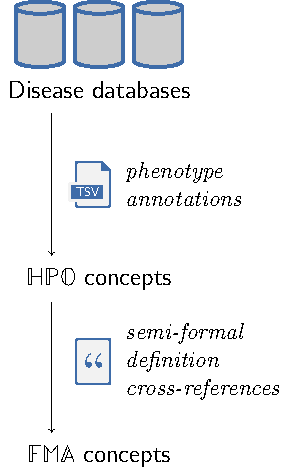
\includegraphics{images/disease2fma.pdf}
    \caption[Workflow to find \ontology{FMA} annotations for some diseases]{The first step is to find the annotations from diseases to \ontology{HPO} concepts, which are provided as \texttt{TSV} files in the \ontology{HPO} website; the second step is to leverage on the cross-references that exist in the textual definitions of the \ontology{HPO} concepts to convert them into \ontology{FMA} concepts. This allows one disease to be associated (\ie annotated) with a set of \ontology{FMA} concepts.}
    \label{fig:disease2fma}
\end{figure}

The positive and negative datasets were then used to perform Receiving Operating Characteristic (ROC) analysis~\citep{Fawcett2006}. This is a common step in classification approaches, summarised as follows:
\begin{enumerate}
    \item Select a threshold~$t$ and create a binary classifier that classifies as positive all the pairs that have $\ferreira>t$ and as negative the other. For each~$t$, we can determine the true positive rate (TPR \mdash fraction of the related concepts correctly classified as related) and false positive rate (FPR \mdash fraction of the unrelated concepts incorrectly classified as related).
    \item The highest threshold results in a TPR of~$0$ and a FPR of~$0$ (all pairs are classified as negative); likewise, the lowest possible threshold results in a TPR of~$1$ and a FPR of~$1$ (all pairs are classified as positive).
    \item Plot the curve defined by the points $(\textrm{FPR}, \textrm{TPR})$ when the threshold varies from the maximum to the minimum. This is known as the ROC curve. The closer the graph approaches the point~$(0, 1)$ (which represents the ideal case where all the positive pairs have a higher relatedness measure than all negative pairs), the better is the measure of relatedness.
    \item \citet{Fawcett2004} proposes a way to repeat this experiment a number of times and to produce an average ROC curve from them (see Algorithm~5 of that paper), which I followed by repeating these steps $10$~times, each time with a different randomly generated negative dataset.
\end{enumerate}

The ROC curves obtained with this method are presented in \figref{fig:roc}. For comparison purposes, I applied the proposed $\ferreira$~measure, calculated for $M=3$ and~$M=4$, and I also applied~$\sim[GIC]$ to the dataset to study how the behaviour of a similarity measure contrasts with the behaviour of a relatedness measure.

\begin{figure}
    \centering
    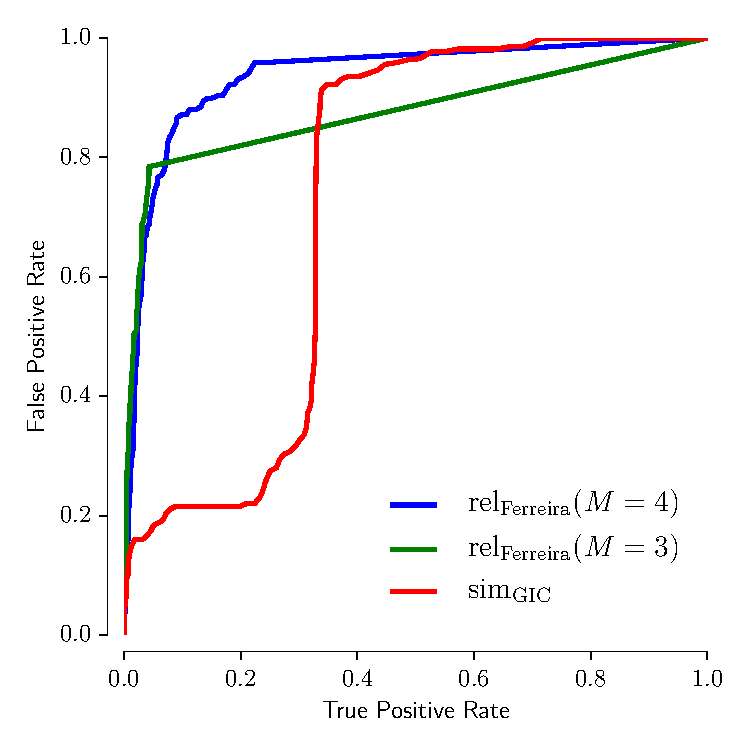
\includegraphics[width=0.8\textwidth]{images/roc.pdf}
    \caption[ROC analysis of the results of~$\ferreira$]{These ROC curves are the average over $10$~runs, each one produced with a different, randomly selected, negative set (\ie randomly selected pairs of \ontology{FMA} concepts).}
    \label{fig:roc}
\end{figure}

As is evident from this figure, $\ferreira$ shows a better performance than $\sim[GIC]$, since high values of TPR are obtained for low values of FPR. The main difference between $\ferreira$ with $M=4$ and~$M=3$ is that the former has more resolution power in that it can differentiate between concepts $8$~properties apart, whereas in the latter concepts with a path distance greater than~$6$ have automatically a relatedness value of~$0.0$. Thus, the measure calculated for many of the negative pairs in the dataset and also some of the positive ones ended up being~$0$. Given the lower resolution of the measure for~$M=3$, more pairs in this setting have relatedness~$0.0$, resulting in the straight diagonal line that we see in the figure.

Additionally, $\sim[GIC]$ does not perform as well as the relatedness measure. The distinct form of the graph occurs because a majority of the positive pairs (\ontology{FMA} concepts implicated in the same disease) are not really similar but simply related, just as in the example above: \term{Heart} and \term{Aortic valve} are relatively frequently implicated in the same disease, and their relatedness is high, as one is part of the other; on the other hand similarity measures are unable to capture this, since one is an organ and the other a valve, two distinct concepts.

This demonstrates the superiority of semantic relatedness measures over semantic similarity, at least when applied to ontologies where there is a vast number of properties, such as \ontology{FMA}, an in contexts where relatedness is more important than mere similarity.


\subsection{Conclusions and future work}

The most important conclusion to take from this work is that measures of relatedness can, in some cases, be more accurate than state-of-the-art measures of similarity, suggesting that relatedness measures do indeed play a role in the biomedical domain, especially when the expressiveness of the relevant ontologies (as measured by the number of properties) is as high as in this case.

The measure that I propose here is based on the concepts of \emph{semantic neighbourhood} and \emph{relevance factors}, and can accommodate the needs of particular applications by fine tuning its parameters. For example, by giving different weights to different properties, the measure can give more importance to some neighbours than others. Machine-learning algorithms can be used to tune the weight of each property according to the needs of each application.

The concept of relevant neighbourhood introduced in this work is also a bridge to other methodologies, particularly in allowing the use of ontology mappings to define wider neighbourhoods that draw not only from a specific ontology but from related ontologies as well, as long as a mapping of some sort exists between them. For example, cross-references can be used for this effect. In this context, the measure can incorporate external knowledge, but is not required to do so. For example, the semantic neighbourhood of a disease can include its symptoms and known treatments; to find the neighbourhood of enzymes, it is possible to include the chemical compounds that they transform; \etc.

Finally, the analysis preformed here on \ontology{FMA} shows that this is a valid method to measure relatedness between biomedical concepts. As we will see later, I have successfully applied this measure to other ontologies and other datasets (see \chpref{chap:multidomain}).


\section{Summary} \label{sec:enhancements/summary}

This chapter delineates my efforts in incorporating OWL axioms other than hypernymy into semantic measures. The first section deals with disjointness axioms while the second with existential quantification axioms. While this is by no means a comprehensive approach to using OWL formalism in semantic similarity, it paves the way for future experimentation and research in this context. As argued by \citet{Couto2013}, increasing the amount of such constructions used in semantic similarity calculations will eventually improve the overall panorama in this field of research and, therefore, the utility of this technique. As such, the results presented here are one of my major contributions to the area of semantic similarity and relatedness.

Even though these results do not directly support the idea of multiple-ontology semantic similarity, they were invaluable to the whole corpus of research that I was committed to achieve. In fact, they represent real scientific advances. Additionally, although $\ferreira$ was not originally validated in a multi-domain context, it can be easily converted into a measure that is able to tackle that problem, as we will see in \chpref{chap:multidomain}, by allowing the semantic neighbourhood of concepts to be generated based on several ontologies.
